%---------------------------------------------------------------------
%
%                          Ap�ndice UML
%       Para poner las im�genes de los dise�os UML
%
%---------------------------------------------------------------------

\chapter{Diagramas UML}
\label{app:UML}


%\begin{resumen}
En este ap�ndice incluimos los diagramas UML que hemos usado durante el dise�o de nuestra aplicaci�n PMCTrack-GUI, y que sin duda, servir�n al lector para un mayor entendimiento del funcionamiento interno de la aplicaci�n.
%\end{resumen}

\clearpage

\begin{landscape}

%-------------------------------------------------------------------
\section{PMCTrack-GUI - Objetos de procesamiento}
%-------------------------------------------------------------------
\label{app:UML.XML}
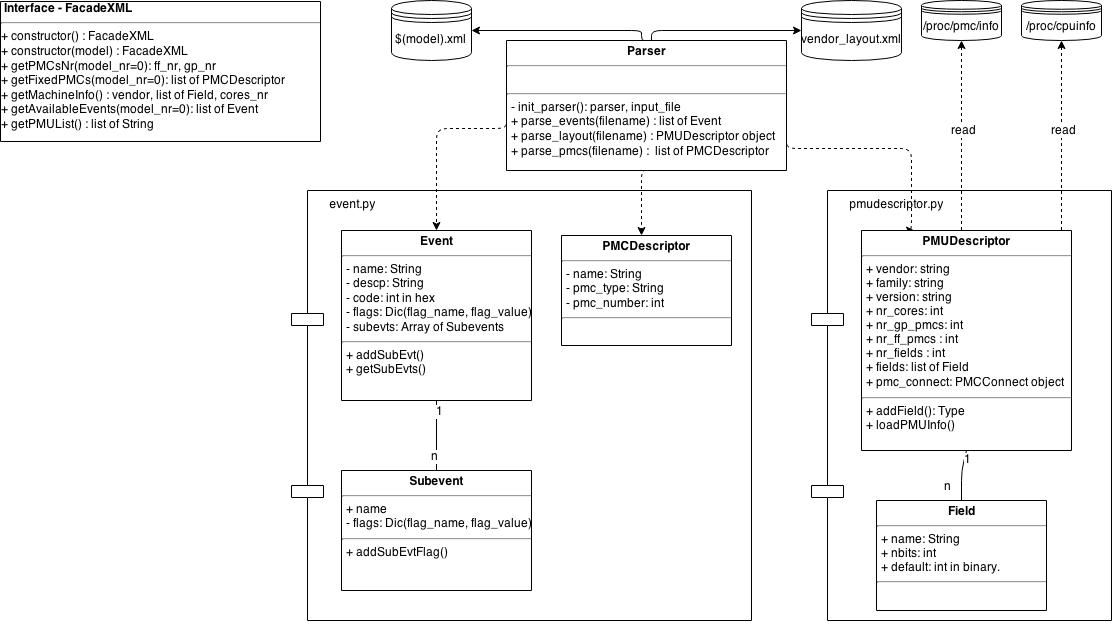
\includegraphics[scale=0.5]{Imagenes/Bitmap/XMLdiagram}

%-------------------------------------------------------------------
\section{PMCTrack-GUI - Objetos de configuraci�n de usuario}
%-------------------------------------------------------------------
\label{app:UML.UserConfig}
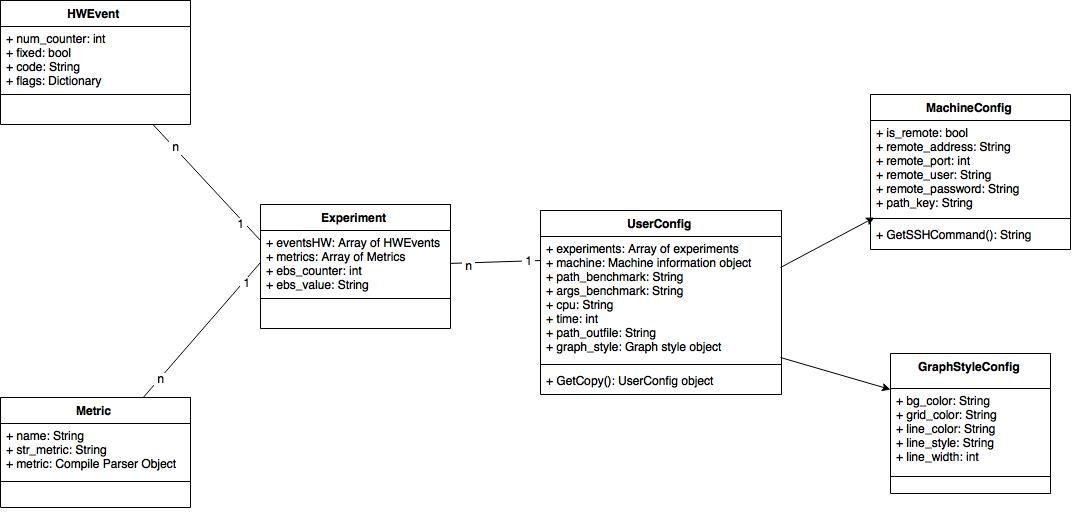
\includegraphics[scale=0.5]{Imagenes/Bitmap/UserConfigDiagram}

\end{landscape}
